\documentclass{standalone}
\usepackage{tikz}
\usepackage{ctex,siunitx}
\setCJKmainfont{Noto Serif CJK SC}
\usepackage{tkz-euclide}
\usepackage{amsmath}
\usetikzlibrary{patterns, calc,3d}
\usetikzlibrary {decorations.pathmorphing,decorations.pathreplacing,decorations.shapes}
\tikzset{label style/.append style={font=\small}}
\begin{document}
\small
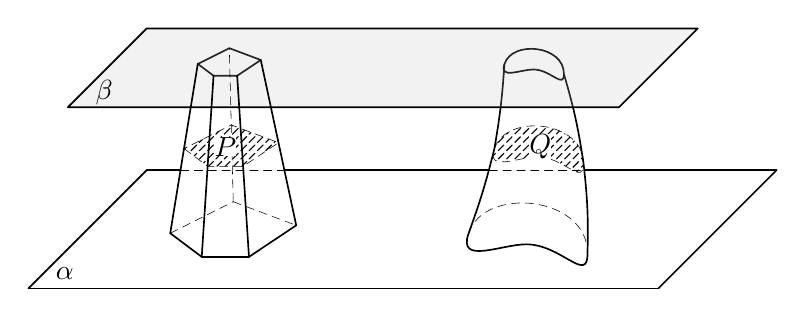
\begin{tikzpicture}[>=latex,scale=1.0]
  \tkzDefPoints{0/0/A,8/0/B,9.5/1.5/C,1.5/1.5/D,5.85/1.5/ll,7.07/1.5/lr}
  \tkzDefPoints{0.5/2.3/A',7.5/2.3/B',8.5/3.3/C',1.5/3.3/D'}
  \tkzDefPoints{1.8/0.7/N1,2.2/0.4/N2,2.8/0.4/N3,3.4/0.8/N4,2.6/1.1/N5,2.5/5/S}
  \foreach \x in {1,...,5}
  {
    \tkzDefMidPoint(S,N\x)\tkzGetPoint{M\x}
    \tkzDefMidPoint(M\x,N\x)\tkzGetPoint{P\x}
  }
  \tkzInterLL(C,D)(N1,M1)\tkzGetPoint{LL}
  \tkzInterLL(C,D)(N4,M4)\tkzGetPoint{LR}
  \tkzDefPoints{6.321/0.559/L1,6.002/0.559/L2,5.449/0.296/L3,5.588/0.695/L4,5.784/1.310/L5,7.107/1.176/L6,7.099/0.442/L7,7.102/0.052/L8,6.763/0.560/L9,6.5/5/H}
   \foreach \x in {1,...,9}
  {
    \tkzDefMidPoint(H,L\x)\tkzGetPoint{K\x}
    \tkzDefMidPoint(K\x,L\x)\tkzGetPoint{Q\x}
    \tkzDefShiftPoint[Q\x](0.1,0){T\x}
  }
  \draw[semithick](K1)..controls(K2)and(K3)..(K4)..controls(K5)and(K6)..(K7)..controls(K8)and(K9)..cycle;

  \draw[densely dashed,very thin](L4)..controls(L5)and(L6)..(L7);
  \draw[semithick](L7)..controls(L8)and(L9)..(L1)..controls(L2)and(L3)..(L4);
  \draw[densely dashed,very thin,pattern=north east lines](T1)..controls(T2)and(T3)..(T4)..controls(T5)and(T6)..(T7)..controls(T8)and(T9)..cycle;
  \draw[semithick](K4)to[bend left=3](T4)to[bend left=3](L4);
  \draw[semithick](K7)to[bend left=4](T7)to[bend left=4](L7);

  \tkzDrawSegments[semithick](D,A A,B B,C LL,D lr,C LR,ll)
  \tkzDrawPolygon[semithick](M1,M2,M3,M4,M5)
  \tkzDrawPolygon[semithick,fill=lightgray,fill opacity=0.2](A',B',C',D')
  \tkzDrawPolygon[densely dashed,pattern=north east lines](P1,P2,P3,P4,P5)
  \tkzDrawSegments[semithick](N1,N2 N2,N3 N3,N4 N1,M1 N2,M2 N3,M3 N4,M4)
  \tkzDrawSegments[densely dashed](N1,N5 N5,N4 N5,M5 LL,LR ll,lr)

  \tkzLabelAngle[pos=0.5](B,A,D){$\alpha$}
  \tkzLabelAngle[pos=0.5](B',A',D'){$\beta$}
  \node at (2.5,1.8)[inner sep=0pt,fill=white]{$P$};
  \node at (6.5,1.8)[inner sep=0pt,fill=white]{$Q$};
\end{tikzpicture}
\end{document}